\documentclass{article}
\usepackage{graphicx}
\usepackage[utf8]{inputenc}
\usepackage{amsmath, amssymb, latexsym}

\usepackage{pgfplots}
\usepackage{algorithm}
\usepackage[noend]{algpseudocode}
\usepackage{tikz}
\usepackage{nicefrac}
\pgfplotsset{every axis legend/.append style={
at={(0,0)},
anchor=north east}}
\usetikzlibrary{shapes,positioning,intersections,quotes}
\usetikzlibrary{arrows.meta,
                bending,
                intersections,
                quotes,
                shapes.geometric}
                
\definecolor{darkgreen}{rgb}{0.0, 0.6, 0.0}
\definecolor{darkred}{rgb}{0.7, 0.0, 0.0}
\makeatletter
\def\BState{\State\hskip-\ALG@thistlm}
\makeatother
\title{Week 14}
\begin{document}
\pagenumbering{gobble}
\maketitle
\newpage
\pagenumbering{arabic}

\section*{Compression}

\begin{itemize}
  \item Speeds up algorithms.
  \item Saves space.
  \item Dimension reduction: not all features are needed.
  \item Example: different units for same attribute.
\end{itemize}

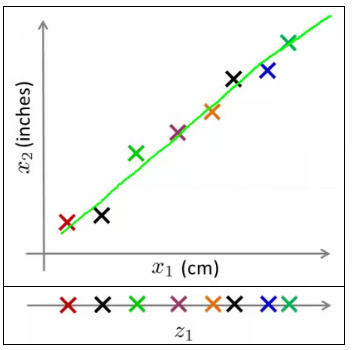
\includegraphics[width=0.5\textwidth]{resources/compression_units}


~\\
Now we can represent x1 as a 1D number (Z dimension).


\section*{Visualization}

\begin{itemize}
  \item It is difficult to visualize higher dimensional data.
  \item Dimensionality reduction can help us show information in a more readable fashion for human consumption.
  \item Collect a huge data set including numerous facts about a country from around the world.
\end{itemize}

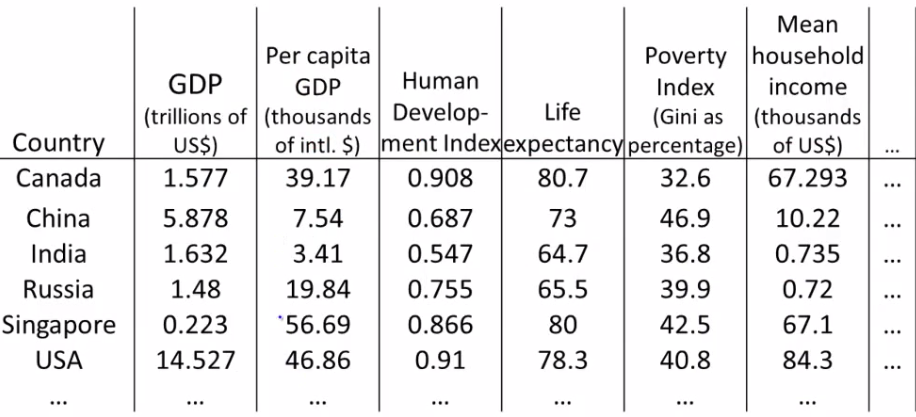
\includegraphics[width=0.8\textwidth]{resources/table}

\begin{itemize}
  \item Assume each country has 50 characteristics.
  \item How can we better comprehend this data?
  \item Plotting 50-dimensional data is quite difficult.
  \item Create a new feature representation (2 z values) that summarizes these features.
  \item Reduce $50D\ ->\ 2D$ (now possible to plot).
\end{itemize}

\section*{Principle Component Analysis (PCA): Problem Formulation}

\begin{itemize}
  \item Assume we have a 2D data collection that we want to reduce to 1D.
  \item How can we choose a single line that best fits our data?
  \item The distance between each point and the projected version should be as little as possible (blue lines below are short).
  \item PCA tries to find a lower dimensional surface so the sum of squares onto that surface is minimized.
  \item PCA tries to find the surface (a straight line in this case) which has the minimum projection error.
\end{itemize}

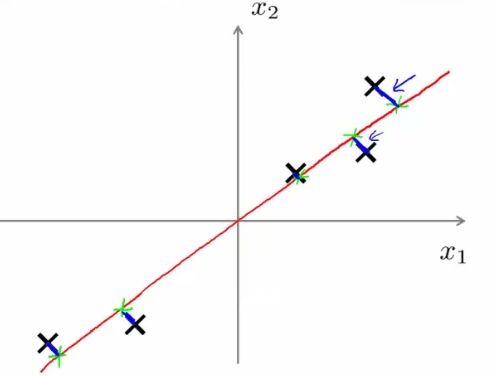
\includegraphics[width=0.5\textwidth]{resources/pca}

\begin{itemize}
  \item PCA is not linear regression.
  \item For linear regression, fitting a straight line to minimize the straight line between a point and a squared line. VERTICAL distance between point.
  \item For PCA minimizing the magnitude of the shortest orthogonal distance.
  \item With PCA there is no $y$ - instead we have a list of features and all features are treated equally.
\end{itemize}

\section*{PCA Algorithm}

\begin{itemize}
  \item Compute the covariance matrix.

        $$\Sigma = \frac{1}{m} \sum_{i=1}^{n} (x^{(i)})(x^{(i)})^T$$
  \item This is an $[n x n]$ matrix (Remember than $x^i$ is a $[n \times 1]$ matrix).
  \item Next, compute eigenvectors of matrix $\Sigma$.
  \item [U,S,V] = svd(sigma)
  \item $U$ matrix is also an $[n \times n]$ matrix. Turns out the columns of $U$ are the u vectors we want!
  \item Just take the first k-vectors from U.
  \item Next, calculate $z$.  $$z = (U_{reduce})^T \cdot x$$
\end{itemize}


\section*{Reconstruction from Compressed Representation}

\begin{itemize}
  \item Is it possible to decompress data from a low dimensionality format to a higher dimensionality format?

        $$x_{approx} = U_{reduce} \cdot z$$

  \item We lose some information (everything is now precisely aligned on that line), but it is now projected into 2D space.
\end{itemize}

\section*{Choosing the number of Principle Components}

\begin{itemize}
  \item PCA attempts to minimize the averaged squared projection error.

        $$\frac{1}{m} \sum_{i=1}^{m} ||x^{(i)} - x_{approx}^{(i)}||^2$$

  \item Total data variation may be defined as the average over data indicating how distant the training instances are from the origin.

        $$\frac{1}{m} \sum_{i=1}^{m} ||x^{(i)}||^2$$

  \item To determine k, we may use the following formula:

        $$\frac{\frac{1}{m} \sum_{i=1}^{m} ||x^{(i)} - x_{approx}^{(i)}||^2}{\frac{1}{m} \sum_{i=1}^{m} ||x^{(i)}||^2} \leq 0.01$$

\end{itemize}

\section*{Applications of PCA}


\begin{itemize}
  \item Compression: Reduce the amount of memory/disk space required to hold data.
  \item Visualization: k=2 or k=3 for plotting.
  \item A poor application of PCA is to avoid over-fitting. PCA discards certain data without understanding what values it is discarding.
  \item Examine how a system works without PCA first, and then apply PCA only if you have reason to believe it will help.
\end{itemize}



\end{document}